\documentclass[tikz,border=2pt]{standalone}
\usepackage{amsmath,amssymb}
\usepackage{tikz}
\usepackage{pgfplots}
\pgfplotsset{compat=1.18}

\begin{document}
% Meals: demand uniform on [80,120], overage h = 2.2, underage b = 3.3. Expected overage cost
% h(y-80)^2/80 rises, expected underage cost b(120-y)^2/80 falls, their sum G(y) is convex
% with minimum 26.4 at y* = 104.
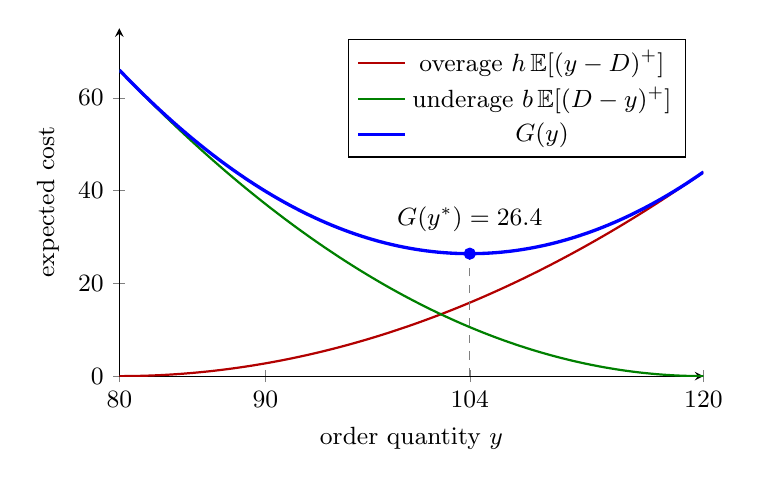
\begin{tikzpicture}
	\begin{axis}[width=9cm, height=6cm, xlabel={order quantity $y$}, ylabel={expected cost}, xmin=80, xmax=120, ymin=0, ymax=75, axis lines=left, legend pos=north east, legend style={font=\small}, tick label style={font=\small}, label style={font=\small}, samples=100, xtick={80,90,104,120}]
		\addplot[red!70!black, thick, domain=80:120] {2.2*(x-80)^2/80};
		\addlegendentry{overage $h\,\mathbb E[(y-D)^+]$}
		\addplot[green!50!black, thick, domain=80:120] {3.3*(120-x)^2/80};
		\addlegendentry{underage $b\,\mathbb E[(D-y)^+]$}
		\addplot[blue, very thick, domain=80:120] {2.2*(x-80)^2/80+3.3*(120-x)^2/80};
		\addlegendentry{$G(y)$}
		\draw[dashed, gray] (axis cs:104,0) -- (axis cs:104,26.4);
		\addplot[only marks, mark=*, mark size=2pt, blue] coordinates {(104,26.4)};
		\node[anchor=south, font=\small] at (axis cs:104,29) {$G(y^*)=26.4$};
	\end{axis}
	\end{tikzpicture}
\end{document}
